\chapter{Preparando o Ambiente de Desenvolvimento}

\section{Introdução}

O desenvolvimento de aplicativos para a plataforma Android é feito na
linguagem Java. Para este guia serão utilizados os seguintes aplicativos
e bibliotecas:

\begin{itemize}
\item
  Ubuntu 14.04
\item
  Java JDK 6 ou 7
\item
  Android SDK
\item
  Android 4.4 API 17 e 2.2 API 8
\item
  Android Studio
\item
  Sqlite3
\item
  Sqliteman
\item
  Inkscape
\end{itemize}
Você pode estar se perguntando: ``Por que utilizar essa configuração?''.
Bom, para começar um ambiente de desenvolvimento precisa ser estável, e
para isso nada melhor que o \url{http://releases.ubuntu.com/trusty/}
(Ubuntu 14.04) por ser \gls{lts}.

A \gls{ide} Android Studio funciona independente do sistema operacional,
então podemos utilizar a versão mais recente.

Usaremos especificamente para os exemplos a seguir as versões 4.4 e 2.2
do Android. Essas \gls{api}'s são uma ótima escolha inicial, pois são as
mais utilizadas pelos aparelhos que rodam Android. É claro que você
poderá instalar outras versões e compilar seus aplicativos para
\emph{tablets}, etc.

\section{Instalação}

\subsection{Java JDK 6}

Para a instalação no Ubuntu 14.04 temos que habilitar um repositório de
terceiros, também conhecidos como \gls{ppa} (Personal Package Archives).
Abra um terminal e execute os passos a seguir para adicionar um
repositório e instalar o Java 6:

\begin{verbatim}
$ sudo su
# apt-add-repository ppa:flexiondotorg/java
# apt-get update
# apt-get install sun-java6-jdk
\end{verbatim}
\subsubsection{Um pouco de Linux}

Para quem não está familiarizado com o ambiente Linux vamos a uma
pequena explicação. Nos comandos acima aparecem dois caracteres que não
devem ser escritos mas que representam algo importante no âmbito dos
comandos, são eles \texttt{\$} e \texttt{\#}. Estes caracteres indicam
qual o nível do usuário; \texttt{\$} significa usuário comum,
\texttt{\#} representa super usuário (\texttt{root}). No comando
\texttt{sudo su} é onde trocamos de usuário comum para super usuário.
Neste momento você terá que entrar com sua senha de \emph{login}.

\subsubsection{Java JDK 7}

Segundo a página de Requerimentos do Sistema
(\url{http://developer.android.com/sdk/requirements.html}) do site
oficial do Android, é necessário uso do Java 6. Caso você queira
utilizar o Java 7, você terá que configurar seu projeto Android para ser
compilado com suporte a versão 6.

A instalação do Java 7 no Ubuntu 14.04 pode ser feita da seguinte
maneira:

\begin{verbatim}
$ sudo su
# add-apt-repository ppa:webupd8team/java
# apt-get update
# apt-get install oracle-jdk7-installer
\end{verbatim}
\subsection{Android Studio}

\begin{figure}[h]
\centering

\includegraphics[scale=0.4]{img/preparando-ambiente/android-studio-splash.png}
\caption{Android Studio splash screen}
\end{figure}

A IDE Android Studio pode ser encontrada em
\url{http://developer.android.com/sdk/installing/studio.html}. É um
ambiente completo de desenvolvimento baseado na IntelliJ IDEA.

O Android Studio não possui instalador, no caso ele já vem
pré-compilado. Basta apenas descompactar e executar o arquivo
\texttt{bin/studio.sh}.

Para sua comodidade você pode adicionar o Android Studio no menu do
Ubuntu. Isso pode ser feito diretamente do Android Studio. Vá até o menu
\texttt{Tools} (ou \texttt{Configure} caso você não tenha nenhum projeto
aberto) $\rightarrow$ \texttt{Create Desktop Entry}. Daí ele pergunta se
é só para o seu usuário ou para todos. Caso escolha para todos ele irá
requisitar sua senha para fazer alterações como \texttt{root}.

Para saber como faz isso manualmente use a dica do blog MAD3 Linux
(\url{http://www.mad3linux.org}) - \url{http://va.mu/VSgR}. Essa dica
irá lhe mostrar como adicionar um item ao menu visível a todos os
usuários.

\subsection{Android SDK \label{ssec:sdk}}

O Android \gls{sdk} já vem junto do Android Studio, sendo assim apenas
instale as API's necessárias. Basta clicar em \texttt{Tools}
$\rightarrow$ \texttt{Android} $\rightarrow$ \texttt{SDK Manager} e
selecionar as versões 4.4 e 2.2.

\subsection{Android Virtual Device (AVD)}

\begin{figure}[h]
    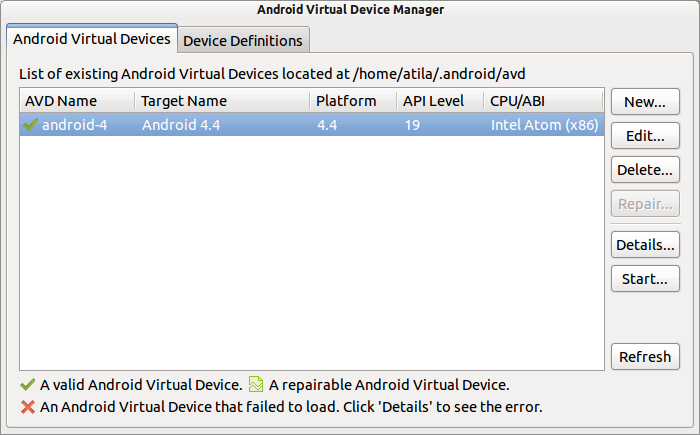
\includegraphics[scale=0.5]{img/preparando-ambiente/android-avd.png}
    \caption{Android AVD}
\end{figure}

Vamos aproveitar e criar nosso \gls{avd} para testar pela primeira vez
nosso emulador. Ainda no Android Studio clique em \texttt{Tools}
$\rightarrow$ \texttt{Android} $\rightarrow$ \texttt{AVD Manager}. Na
aba \texttt{Android Virtual Devices} clique em \texttt{New...}

Dê um nome. Você pode usar qualquer nomenclatura, mas é interessante que
tenha algo haver com a versão. Assim, caso você tenha que testar seu
código em outras versões você poderá saber qual emulador utilizar. Por
exemplo use \texttt{android-4.4}. Em \texttt{Target} escolha a versão,
neste caso \texttt{Android 4.4 (API 19)}. Pronto, apenas clique em
\texttt{Create AVD}.

\subsubsection{Dicas}

A opção \texttt{Device} indica qual a resolução da tela do aparelho.
Como não é possível redimensionar a janela, em alguns monitores a janela
fica maior que a tela do seu monitor.

A opção \texttt{Snapshot} quando habilitada, serve para salvar o estado
do emulador. Isso faz com que da segunda inicialização em diante se
torne mais rápida.

A opção \texttt{SD Card} é ideal caso sua aplicação necessite guardar
dados como fotos, arquivos. O AVD irá reservar um espaço em seu HD
permitindo assim o acesso a dados pelo emulador.

\subsubsection{Primeiro projeto Android \label{sssec:testando}}

Para criar um projeto no Android Studio selecione \texttt{File}
$\rightarrow$ \texttt{New Project...}

Dê um nome qualquer ao seu aplicativo, por exemplo
\texttt{hello.android}. Note que o Android Studio tenta dar um nome ao
seu pacote e ao diretório de arquivos a partir do nome que você digitou.
Deixe como está. Em \texttt{Target SDK} é preciso escolher qual API
vamos utilizar, em nosso caso escolha a \texttt{API 19: Android 4.4}. Em
\texttt{Minimum Required SDK} escolha a
\texttt{API 8: Android 2.2 (Froyo)} indicando que a versão mínima é a
\texttt{API 8}. Clique em \texttt{Next}.

É possível criar o ícone lançador logo ao criar o aplicativo. Selecione
da maneira que achar melhor e clique em \texttt{Next}. Em seguida temos
a tela inicial do projeto, a opção \texttt{Blank Activity} vem
selecionado por padrão, clique em \texttt{Next}. Por fim clique em
\texttt{Finish}.

Após isso basta executar o projeto usando \texttt{Shift + F10} ou no
menu \texttt{Run} $\rightarrow$ \texttt{Run 'main'}. Se tudo tiver dado
certo é possível ver no emulador sua primeira aplicação rodando.

\subsubsection{Dicas}

Uma vez que você abriu o emulador não o feche. Você irá notar que ao
abrir pela primeira vez ele leva um tempo para isso. Neste caso ao
atualizar o código-fonte apenas rode o aplicativo novamente. O plugin
ADT fará com que o aplicativo seja reinstalado no emulador.

Faça o teste com alguns atalhos básicos:

\begin{itemize}
\item
  \textbf{\texttt{Alt + Enter}} Maximiza o emulador. Ideal para
  demostrações.
\item
  \textbf{\texttt{Ctrl + F11}} Muda a orientação do emulador, retrato ou
  paisagem.
\item
  \textbf{\texttt{F8}} Liga/desliga a rede.
\end{itemize}
Para mais detalhes acesse
\url{http://developer.android.com/tools/help/emulator.html#KeyMapping}

Outro elemento essencial é o \texttt{LogCat}. Ele é responsável por
mostrar as mensagens de \emph{log} do emulador. Caso você encontre
problemas com seu código o \texttt{LogCat} será seu melhor aliado. Para
acessá-lo utilize o atalho \texttt{Alt + 6}.

\subsection{Sqlite3}

Sendo o Sqlite o banco de dados embutido na plataforma Android, nada
melhor do que aprendermos um pouco sobre ele.

O Sqlite é um banco de dados relacional bastante utilizado por
dispositivos e sistemas embarcados por ser leve, robusto, de fácil
configuração e, acima de tudo, livre. Para a instalação, abra um
terminal como \texttt{root} e:

\begin{verbatim}
$ sudo su
# apt-get install sqlite3
\end{verbatim}
Após a instalação é possível utilizar o Sqlite via linha de comando.
Faça \emph{logoff} do usuário \texttt{root} e faça os seguintes testes:

\begin{verbatim}
# exit
$ sqlite
SQLite version 2.8.17
Enter ".help" for instructions
sqlite>
\end{verbatim}
Você deverá ver algo parecido. Para sair utilize o comando
\texttt{.exit}. Veja outros detalhes na página oficial do projeto:
\url{http://www.sqlite.org/}.

\subsubsection{Tipos de dados}

Utilize a tabela abaixo para criar suas tabelas futuramente.

\ctable[caption = Tipos de dados do Sqlite, pos = H, center, botcap]{ll}
{% notes
}
{% rows
\FL
\parbox[b]{0.14\columnwidth}{\raggedright
\textbf{Nome}
} & \parbox[b]{0.86\columnwidth}{\raggedright
\textbf{Descrição}
}
\ML
\parbox[t]{0.14\columnwidth}{\raggedright
\texttt{INTEGER}
} & \parbox[t]{0.86\columnwidth}{\raggedright
valores inteiros, positivos ou negativos. Podem variar de 1 a 8
\emph{bytes}.
}
\\\noalign{\medskip}
\parbox[t]{0.14\columnwidth}{\raggedright
\texttt{REAL}
} & \parbox[t]{0.86\columnwidth}{\raggedright
valores reais ou decimais.
}
\\\noalign{\medskip}
\parbox[t]{0.14\columnwidth}{\raggedright
\texttt{TEXT}
} & \parbox[t]{0.86\columnwidth}{\raggedright
usado para armazenar valores, não-limitado. Suporta várias codificações,
por exemplo \texttt{UTF-8}.
}
\\\noalign{\medskip}
\parbox[t]{0.14\columnwidth}{\raggedright
\texttt{BLOB}
} & \parbox[t]{0.86\columnwidth}{\raggedright
objetos binários tais como imagens, arquivos de texto, etc. Também
possui tamanho não-limitado.
}
\\\noalign{\medskip}
\parbox[t]{0.14\columnwidth}{\raggedright
\texttt{NULL}
} & \parbox[t]{0.86\columnwidth}{\raggedright
representa falta de informação.
}
\LL
}

\subsection{Sqliteman}

\begin{figure}[h]
\centering
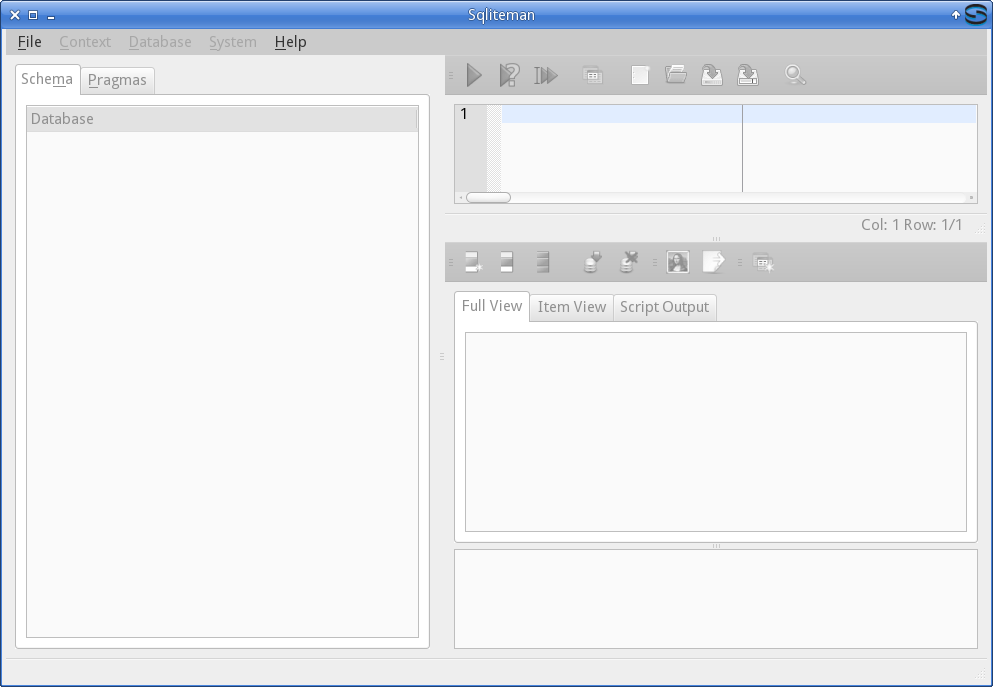
\includegraphics[scale=0.4]{img/preparando-ambiente/sqliteman.png}
\caption{Sqliteman}
\end{figure}

Para uma gerência mais produtiva usaremos o Sqliteman para acessar e
modificar bancos de dados. A instalação é feita via linha de comando.
Abra um terminal e:

\begin{verbatim}
$ sudo su
# apt-get install sqliteman
\end{verbatim}
Depois de instalado, acesse o aplicativo do menu principal do Ubuntu em
\texttt{Aplicativos} $\rightarrow$ \texttt{Escritório} $\rightarrow$
\texttt{Sqliteman}. Faça alguns testes criando bancos de dados, depois
crie algumas tabelas. Ele possui assistentes que irão auxiliar nos
primeiros momentos.

Por exemplo, crie uma base de dados e depois clique com o botão direito
do \emph{mouse} em \texttt{Tables}. Utilize o assistente e veja como é
simples criar tabelas no sqlite.

\begin{listing}[H]
  \inputminted[linenos=true,frame=bottomline,tabsize=3]{ sql }{ source/exemplo-bd-1.sql }
  \caption{Exemplo de banco de dados [exemplo-bd.sql]}
\end{listing}

Observe que podemos fazer auto-relacionamento na tabela. Assim somos
capazes de executar a seguinte SQL, contando o número de distros que
derivam de uma outra original. Veja:

\begin{listing}[H]
  \inputminted[linenos=true,frame=bottomline,tabsize=3]{ sql }{ source/exemplo-bd-2.sql }
  \caption{Exemplo de \textit{query} com \textit{subquery} [exemplo-bd.sql]}
\end{listing}

Mais informações em: \url{http://sqliteman.com/}

\subsection{Inkscape}

\begin{figure}[h]
\centering
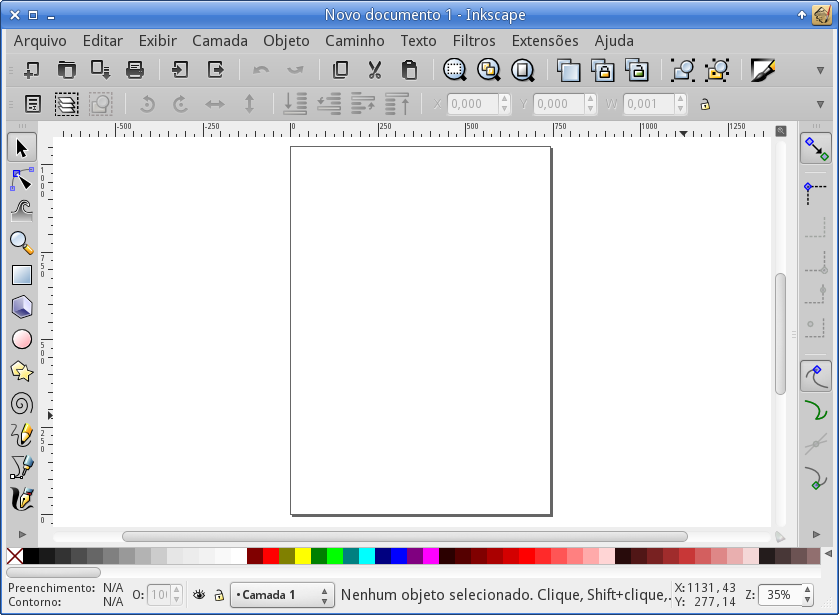
\includegraphics[scale=0.45]{img/preparando-ambiente/inkscape.png}
\caption{Inkscape}
\end{figure}

Uma ótima ferramenta de desenho vetorial é o Inkscape. Ela será bastante
útil pois o desenvolvimento de aplicativos hoje em dia é baseado muito
em figuras para facilitar a navegação, identidade visual, entre outras
coisas.

A instalação é feita de forma simples. Num terminal:

\begin{verbatim}
$ sudo su
# apt-get install inkscape
\end{verbatim}
Para dicas de como criar ícones para os diversos elementos do Android
veja a página
\url{http://developer.android.com/design/style/iconography.html}.

\begin{figure}[h]
    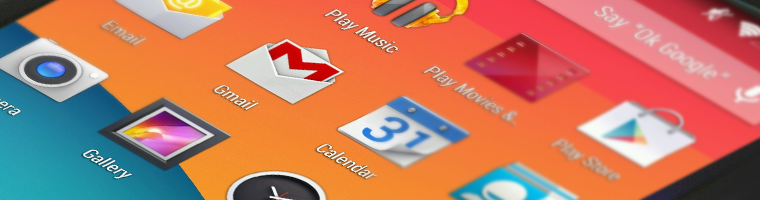
\includegraphics[scale=0.5]{img/preparando-ambiente/iconography-overview.png}
    \caption{Visão geral da iconografia do Android}
\end{figure}
